\section{Synthetic Experiments}

In this section we describe our results on extensive synthetic experiments performed with our model and benchmark methods in two conditions:
1) views missing at random for each dataset,
and 2) datasets with systematically missing views (missing not at random).

%%%%%%%%%%%%%%%%%%%%%%%%%%%
%% SYNTHETIC EXPERIMENTS %%
%%%%%%%%%%%%%%%%%%%%%%%%%%%
\subsection{Data preparation}
\label{ssec:synth}

To simulate multi dataset observations, we sample the latent variable $\z_{d,n}$ from a multivariate Gaussian with zero-mean and identity covariance matrix, and then we transform it with random linear mapping towards the observation space to get $\xdnv$.
We then corrupt the observation with increasing levels of noise
and we apply specific strategies to remove views in the context of the \textit{missing at random} (MAR) and \textit{missing not at random} (MNAR) experiments.

%% MAR %%
In the MAR experiments views were randomly removed according to a parameter $0 \leq f \leq 1$ to control the fraction of data-points with complete views.
In the extreme case $f=1$, all the data-points have all the views, representing the ideal case of no missing views, that is the working case of the Multi-Channel Variational Autoencoder \citep{Antelmi2019}.
In the case $f=0$, each data-point has only one randomly assigned view, representing the case where no relationship between views can be established, where the our multi-view model collapses to a disjoint series of independent Variational Autoencoders \citep{Kingma2013, Rezende2014}.
In the general case, each data-point has probability $f$ to have all the views, and probability $1-f$ to have a randomly assigned view out of the total available views.
The general case represents the case where the relationship between views can be established only through a fraction $f$ of the total available data-points.

%% MNAR %%
In the MNAR experiments we removed specific views for each simulated dataset, ensuring at the same time the absence of at least one view for a datasets, and the presence of at least one view in common between pairs of datasets.
As an example, in the case with three datasets and three views, the association view-dataset can be expressed through the following association matrix $A$:
\begin{equation}
A = 
\begin{pmatrix}
1 & 0 & 1 \\
1 & 1 & 0 \\
0 & 1 & 1 
\end{pmatrix},
\end{equation}
where $A(v,d)=1$ indicates the presence of view $v$ in dataset $d$.
We limited our MNAR simulations to cases with square association matrices with maximum dimensionality of $5$.

\subsection{Model Fitting and Evaluation}

In both MAR and MNAR experiments we fit the synthetic scenarios with our model, where we choose a linear Gaussian parametrization for the variational and likelihood distributions, such that respectively:
\begin{align}
\label{eq:encoder}
q_{d,n,w}(\z) &= \Gaussof{\mub=\mathbf{V}_w^{(\mu)} \xdnw, \Sigmab = diag(\mathbf{V}_w^{(\sigma)} \xdnw)}, \\
\label{eq:decoder}
\p{\xdnv|\z,\thetab_v} &= \Gaussof{\mub = \mathbf{G}_v^{(\mu)} \zb, \Sigmab = diag(\mathbf{g}_v^{(\sigma)})},
\end{align}
\textit{i.e.} factorized multivariate Gaussian distributions whose moments are linear transformations depending on the conditioning variables. \\
$\thetab_v = \{\mathbf{G}_v^{(\mu)}, \mathbf{g}_v^{(\sigma)}\}$ and $\phib_w=\{\mathbf{V}_w^{(\mu)}, \mathbf{V}_w^{(\sigma)}\}$ are the parameters to be optimized through (\ref{eq:argmax}).
Lastly we predicted for each simulated scenario the missing views according to \eqnref{eq:reconstruction} on testing hold-out datasets.

Results, cross validated $5$ times, were summarized with the \textit{mean squared error} (MSE) metric on testing hold-out datasets for every simulated scenario.
We applied the same evaluation procedure for the following benchmark methods.

\subsection{Benchmark Methods}
Among state of the art multivariate linear and non linear imputation methods, we selected the following competitors as a benchmark:
1) k-Nearest Neighbors (knn) with $k=\set{1, 5}$;
2) Denoising Autoencoder (DAE);
3) Multivariate Imputation by Chained Equations (MICE).

For the knn approach we used the \textit{KNNImputer} method as implemented in the \textit{Scikit-Learn} library \citep{sklearn}.
Here each sample's missing values are imputed using the mean value from $k$ nearest neighbors found in the training set.
Two samples are close if the features that neither is missing are close in terms of Euclidean distance.

The Denoising Autoencoder, as developed by \cite{dae}, is based on an overcomplete deep autoencoder.
It maps input data to a higher dimensional subspace, which in combination with an initial dropout layer to induce corruption, makes the model robust to missing data.
We used the same architecture proposed by the authors, that is three hidden layers for encoder and decoder networks, Tanh activation functions, hyperparameter $\Theta=7$, and dropout $p=0.5$, as they proved to provide consistent better results.

In MICE, as implemented in \cite{mice}, missing values are modeled as a multivariate linear combination of the available features.
This methodology is attractive if the multivariate distribution is a reasonable description of the data, which in our case it is by construction.
MICE specifies the multivariate imputation model on a variable-by-variable basis by a set of conditional densities, one for each incomplete variable.
Starting from an initial imputation, MICE draws imputations by iterating over the conditional densities.

\subsection{Results}
\begin{figure}[htb]
\centering
\begin{subfigure}{.49\textwidth}
	\centering
        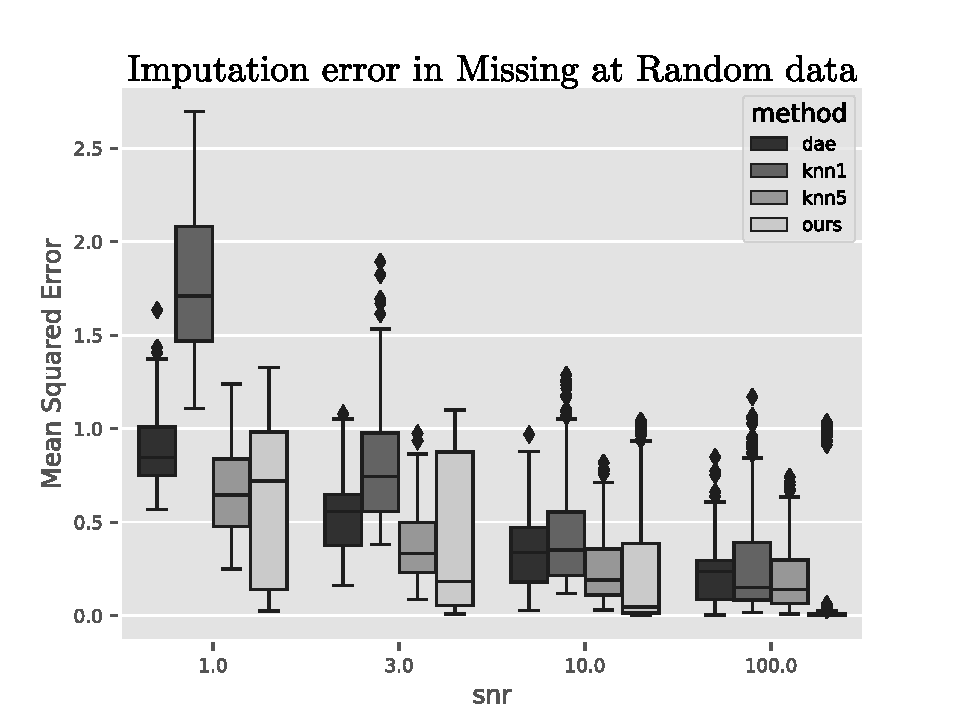
\includegraphics[width=\textwidth]{./tex/fig/mar_imput_err_boxplot.pdf}
        \caption{Missing at random}
        \label{fig:synthetic_benchmark_mar_box}
\end{subfigure}%
\hfill
\begin{subfigure}{.49\textwidth}
	\centering
        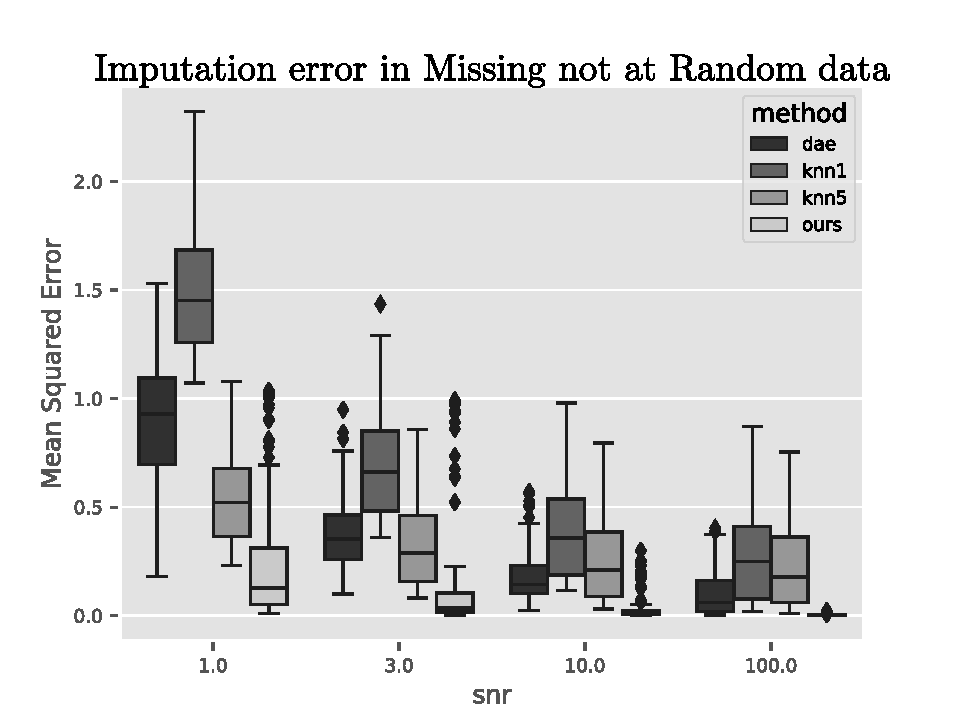
\includegraphics[width=\textwidth]{./tex/fig/mnar_imput_err_boxplot.pdf}
        \caption{Missing not at random}
        \label{fig:synthetic_benchmark_mnar_box}
\end{subfigure}
\caption{
Mean Squared Error of imputation in synthetic datasets. Effect of signal-to-noise ratio (\snr) is shown.
}
\label{fig:synthetic_benchmark_box}
\end{figure}

\begin{figure}[htb]
\centering
\begin{subfigure}{.49\textwidth}
	\centering
        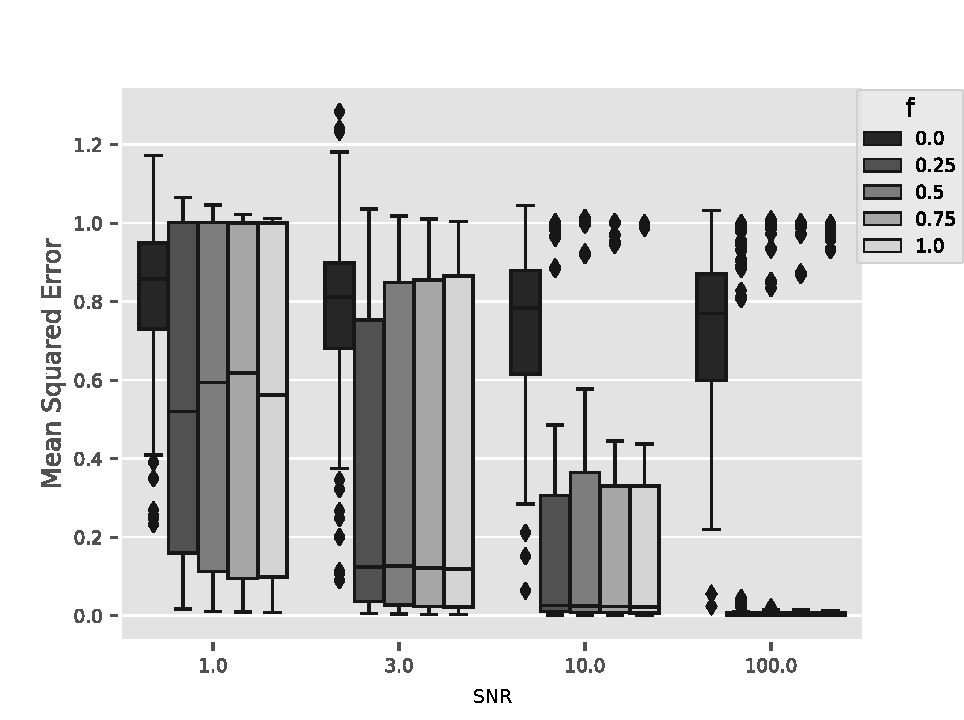
\includegraphics[width=\textwidth]{./tex/fig/mar_pred_err_boxplot.pdf}
        % \caption{Missing at random}
        % \label{fig:synthetic_benchmark_mar_pred_box}
\end{subfigure}%
\caption{
Mean Squared Error of test sets predictions in synthetic datasets.
We show how with already $f \geq 0.25$ (the fraction of observations with all the views) we can significantly reduce the prediction error on testing data-points.
}
\label{fig:synthetic_benchmark_pred_box}
\end{figure}
% \begin{figure}[htb]
% \centering
% \begin{subfigure}{.45\textwidth}
%       \centering
%         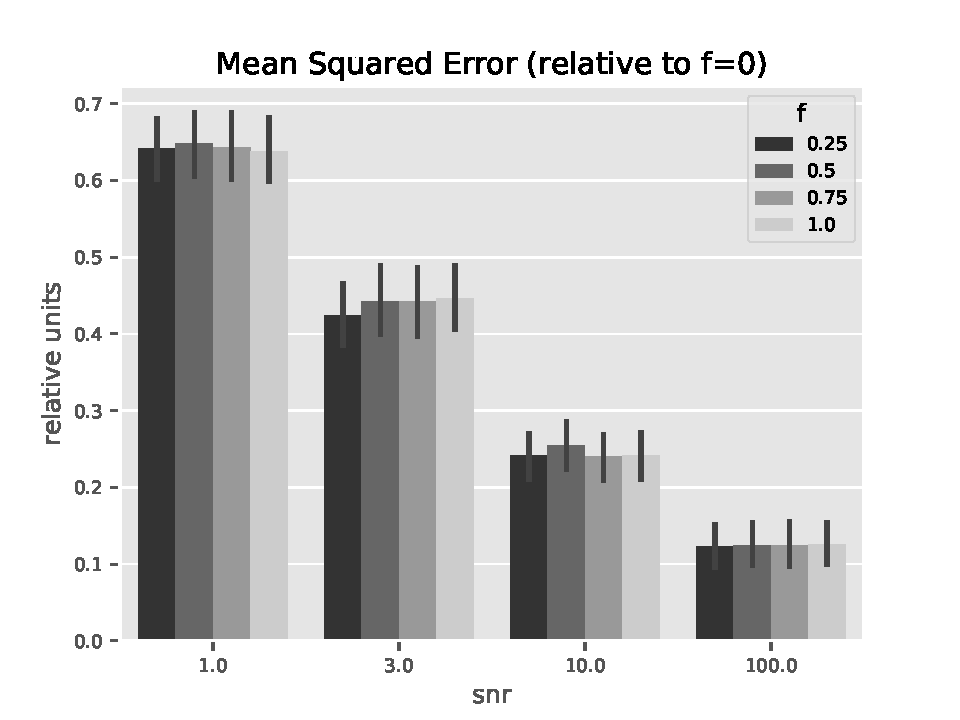
\includegraphics[width=\textwidth]{./tex/fig/mar_barplot.pdf}
%         \caption{Missing at random}
%         \label{fig:synthetic_benchmark_mar_bar}
% \end{subfigure}%
% \hfill
% \begin{subfigure}{.45\textwidth}
%       \centering
%         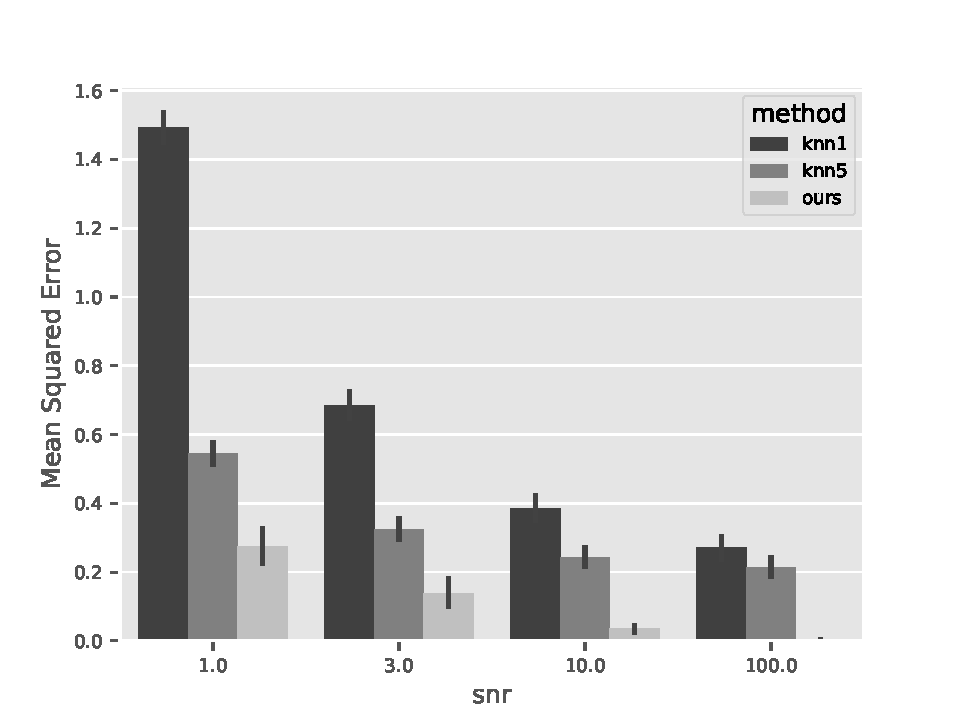
\includegraphics[width=\textwidth]{./tex/fig/mnar_barplot.pdf}
%         \caption{Missing not at random}
%         \label{fig:synthetic_benchmark_mnar_bar}
% \end{subfigure}
% \caption{
% Mean Squared Error of test sets predictions in synthetic datasets. Effect of signal-to-noise ratio (\snr) is shown.
% (a) With $f$ being the fraction of observation with complete views, we show how with already $f \geq 0.25$ we can significantly reduce the prediction error on testing data-points.
% (b) In multi-view datasets where none of the data-point have all the views, and where the available views depends on the specific dataset, we show the prediction performance of our model in comparison with classic k-nearest-neighbors imputation methods.
% }
% \label{fig:synthetic_benchmark_bar}
% \end{figure}



In the synthetic tests our model comes out as the best performer, with a mean MSE improvement compared to best competing method of $17\%$ in MAR cases and $71\%$ in MNAR cases (\figref{fig:synthetic_benchmark_box}).

We notice that DAE is not always better than knn ($k=5$), especially in low \snr\ cases.

Since MICE is computationally expensive, we were able to fit it only on MNAR cases with high \snr\, where it performed poorly (boxplot not shown), while in MAR cases this model did not converge.

In \figref{fig:synthetic_benchmark_pred_box} we show a stratification of MAR experiments results by the fraction $f$ of data-points with complete views.
Here we notice how with already $f \geq 0.25$ we can significantly reduce the prediction error on testing data-points compared to the case $f=0$, where no relationship between views can be established.
Moreover, reaching the ideal case of $f=1$, that is when there are no missing views in the dataset, does not improve significantly the prediction performance of our model.
This finding suggests that collecting a minimum amount of data-points with all the views is enough for our model to capture the joint relationship among views.

%%%%%%%%%%%%%%%%%%%%%
%% MEDICAL IMAGING %%
%%%%%%%%%%%%%%%%%%%%%
\section{Experiments on Medical Imaging Datasets}
\label{ssec:real}

\begin{table}[!t]
\caption{
Number of subjects per view available in each dataset.
The last columns provide the size of the intersection ($\cap$) and union ($\cup$) of subjects with available views.
The mri from the local dataset is considered as a stand-alone modality as the measures were obtained with a different protocol from the ones in the other datasets.
Notice how in the jont dataset no subject have all the modalities.
}
\centering
\resizebox{\columnwidth}{!}{
\begin{tabular}{lccccc|cc}
\toprule
View:          &  clin &   MRI &  FDG & AV45 &  TAU & $\cap$ & $\cup$ \\
\midrule
Dataset \\
adni1          &   740 &   730 &    - &    - &    - & 730 &  740 \\
adni2          &  1324 &   710 &  424 &  417 &   61 &  53 & 1324 \\
miriad         &    67 &    67 &    - &    - &    - &  67 &   67 \\
oasis3         &   529 &   489 &    - &  148 &    - & 147 &  529 \\
geneva         &   999 &     - &   65 &  120 &   54 &  15 &  999 \\
\midrule
Tot. subjects  &  3659 &  1996 &  489 &  685 &  115 &   0 & 3659 \\
\midrule
Tot. datasets  & 5     & 4     & 2    & 3    & 2    &     &      \\
\bottomrule
\end{tabular}}
\label{table:datasets}
\end{table}

% \newpage
% \begin{table}[!t]
\caption{
Mean Squared Error on unseen test data, $5$-fold cross validation.
Mean (standard deviation) across folds are shown. Best results in boldface.
Test data may belong to the same datset used to train the model (within) or on all the other (cross).
Every modality was predicted from the other available ones.
}
\centering
\begin{tabular}{llcccccc}
\toprule
             &       &         clin &          mri &          fdg &         av45 &          tau &   mri local \\
train & test &              &              &              &              &              &              \\
\midrule
adni1 & within &  0.91 (0.11) &  0.95 (0.13) &            - &            - &            - &            - \\
             & cross &  0.91 (0.29) &  1.01 (0.44) &            - &            - &            - &            - \\
\midrule
adni2 & within &  0.77 (0.11) &  \textbf{0.91} (0.20) &  \textbf{0.82} (0.20) &  \textbf{0.93} (0.22) &  1.20 (0.71) &            - \\
             & cross &  0.82 (0.27) &  1.00 (0.41) &            - &  1.28 (0.46) &  1.67 (1.19) &            - \\
\midrule
miriad & within &  0.74 (0.34) &  1.01 (0.52) &            - &            - &            - &            - \\
             & cross &  0.89 (0.15) &  0.99 (0.18) &            - &            - &            - &            - \\
\midrule
local & within &  0.94 (0.28) &            - &            - &  1.20 (0.28) &  1.43 (1.29) &  \textbf{1.23} (0.35) \\
             & cross &  1.29 (0.28) &            - &            - &  1.13 (0.24) &  \textbf{1.17} (0.75) &            - \\
\midrule
\midrule
average & within &  0.84 (0.21) &  0.96 (0.29) &  \textbf{0.82} (0.20) &  1.06 (0.25) &  1.32 (1.00) &  \textbf{1.23} (0.35) \\
        & cross  &  0.98 (0.25) &  1.00 (0.34) &            - &  1.21 (0.35) &  1.42 (0.97) &            - \\
\midrule
\midrule
% all (dae)        & within &  0.56 (0.05) &  1.02 (0.12) &  0.98 (0.24) &  1.02 (0.17) &  1.11 (0.62) &  1.10 (0.34) \\
% all (knn5)        & within &  \textbf{0.65} (0.04) &  1.03 (0.11) &  1.09 (0.20) &  1.42 (0.17) &  1.29 (0.66) &  \textbf{1.23} (0.38) \\
all       & joint &  \textbf{0.65} (0.05) &  0.95 (0.12) &  0.85 (0.21) &  0.99 (0.20) &  \textbf{1.17} (0.64) &  1.25 (0.35) \\
\bottomrule
\end{tabular}
\label{table:crossvalidation_details}
\end{table}

%\begin{table}[!t]
%\caption{
%Same as above, after average-pooling af means and standard deviations by 
%}
%\centering
%\begin{tabular}{lcccccc}
%\toprule
%{} &         clin &          mri &          fdg &         av45 &          tau &   mri local \\
%train/test   &              &              &              &              &              &              \\
%\midrule
%within &  0.84 (0.21) &  0.96 (0.29) &  0.82 (0.20) &  1.06 (0.25) &  1.32 (1.00) &  1.23 (0.35) \\
%cross  &  0.98 (0.25) &  1.00 (0.34) &            - &  1.21 (0.35) &  1.42 (0.97) &            - \\
%joint  &  0.65 (0.05) &  0.95 (0.12) &  0.85 (0.21) &  0.99 (0.20) &  1.17 (0.64) &  1.25 (0.35) \\
%\bottomrule
%\end{tabular}
%\label{table:crossvalidation}
%\end{table}


% \newpage
% \begin{sidewaystable}
\centering
\begin{tabular}{llllllll}
\toprule
       &      &         clin &           mri &          fdg &         av45 &          tau &   mri\_geneva \\
test dataset & train type &              &               &              &              &              &              \\
\midrule
adni1 & within &  0.90 (0.12) &   0.95 (0.16) &            - &            - &            - &            - \\
       & cross &  1.17 (0.80) &   2.88 (3.10) &            - &            - &            - &            - \\
       & lodo &  0.46 (0.07) &   1.13 (0.16) &            - &            - &            - &            - \\
\midrule
adni2 & within &  0.78 (0.12) &   0.91 (0.24) &  0.85 (0.25) &  0.94 (0.27) &  1.24 (0.93) &            - \\
       & cross &  1.08 (0.64) &   2.17 (2.12) &  4.03 (0.85) &  3.34 (2.65) &  1.33 (0.97) &            - \\
       & lodo &  0.60 (0.29) &   0.81 (0.21) &  3.90 (0.90) &  3.04 (2.52) &  1.10 (0.74) &            - \\
\midrule
miriad & within &  0.76 (0.47) &   1.01 (0.66) &            - &            - &            - &            - \\
       & cross &  7.20 (5.07) &  10.39 (4.47) &            - &            - &            - &            - \\
       & lodo &  2.32 (0.95) &   7.97 (2.14) &            - &            - &            - &            - \\
\midrule
geneva & within &  0.89 (0.33) &             - &  1.15 (0.47) &  1.25 (0.37) &  1.86 (3.04) &  1.20 (0.47) \\
       & cross &  2.69 (1.28) &             - &  6.09 (1.95) &  2.57 (3.04) &  2.36 (2.34) &            - \\
       & lodo &  1.83 (0.90) &             - &  5.99 (1.81) &  1.63 (0.48) &  2.47 (2.51) &            - \\
\midrule
oasis3 & within &  0.71 (0.15) &   0.81 (0.11) &            - &  1.10 (0.42) &            - &            - \\
       & cross &  1.29 (0.74) &   2.43 (2.47) &            - &  1.56 (0.93) &            - &            - \\
       & lodo &  0.76 (0.08) &   0.77 (0.11) &            - &  1.74 (0.34) &            - &            - \\
\bottomrule
       & within &  0.81 (0.24) &  0.92 (0.29) &  1.00 (0.36) &  1.10 (0.35) &  1.55 (1.98) &  1.20 (0.47) \\
       & cross  &  2.69 (1.71) &  4.47 (3.04) &  5.06 (1.40) &  2.49 (2.21) &  1.85 (1.66) &            - \\
       & lodo   &  1.19 (0.46) &  2.67 (0.66) &  4.94 (1.35) &  2.14 (1.11) &  1.79 (1.63) &            - \\
\bottomrule
\end{tabular}
\end{sidewaystable}

\begin{table*}
\centering
\caption{
Mean Squared Error (MSE, the lower the better) measured on test dataset views (clinical scores and imaging derived phenotypes) predicted with our model.
$5$-folds cross-validation results shown as as average (standard deviation).
Models were trained on all the available views in the training dataset, independently of their presence in the testing dataset.
Experiments run in three different conditions depending on the provenance of the training data:
1) `same' dataset as the testing dataset;
2) `different' from the testing dataset (average MSE shown);
3) `leave out test', from all the available datasets except the testing dataset.
By average pooling the results (bottom) we see how in general training on data coming from multiple datasets ameliorates the results.
}
\label{tab:features}
\begin{tabular}{llcccccc}
\toprule
       &      &         clin &           mri &          fdg &         av45 &          tau &   mri local \\
test dataset & train dataset &              &               &              &              &              &              \\
\midrule
adni1  & same           &  0.94 (0.11) &  0.83 (0.10) &            - &            - &            - &            - \\
       & different (avg)    &  0.79 (0.26) &  0.78 (0.14) &            - &            - &            - &            - \\
       & leave out test &  0.47 (0.09) &  0.83 (0.13) &            - &            - &            - &            - \\
\midrule
adni2  & same           &  0.78 (0.16) &  0.68 (0.12) &  0.60 (0.10) &  0.81 (0.12) &  1.29 (0.54) &            - \\
       & different (avg)    &  0.68 (0.29) &  0.73 (0.16) &  1.13 (0.17) &  1.04 (0.27) &  1.10 (0.38) &            - \\
       & leave out test &  0.43 (0.07) &  0.69 (0.11) &  1.14 (0.20) &  0.91 (0.17) &  1.03 (0.37) &            - \\
\midrule
miriad & same           &  2.90 (1.24) &  6.19 (1.52) &            - &            - &            - &            - \\
       & different (avg)    &  5.77 (3.83) &  6.32 (1.54) &            - &            - &            - &            - \\
       & leave out test &  1.91 (1.26) &  5.81 (1.35) &            - &            - &            - &            - \\
\midrule
oasis3 & same           &  0.68 (0.24) &  0.65 (0.12) &            - &  1.30 (0.36) &            - &            - \\
       & different (avg)    &  0.98 (0.40) &  0.79 (0.19) &            - &  1.15 (0.32) &            - &            - \\
       & leave out test &  0.74 (0.10) &  0.78 (0.14) &            - &  1.11 (0.32) &            - &            - \\
\midrule
local  & same           &  1.07 (0.43) &            - &  3.23 (1.01) &  1.70 (0.46) &  1.36 (0.77) &  1.36 (0.36) \\
       & different (avg)    &  2.49 (1.30) &            - &  2.70 (0.76) &  1.52 (0.57) &  1.67 (0.78) &            - \\
       & leave out test &  1.76 (1.09) &            - &  2.71 (0.79) &  1.37 (0.38) &  1.49 (0.69) &            - \\
\midrule
\midrule
average& same           &  1.27 (0.60) &  2.09 (0.77) &  \textbf{1.91} (0.72) &  1.27 (0.34) &  1.32 (0.67) &  1.36 (0.36) \\
       & different (avg)    &  2.14 (1.83) &  2.16 (0.78) &  1.92 (0.55) &  1.24 (0.41) &  1.39 (0.61) &            - \\
       & leave out test &  \textbf{1.06} (0.75) &  \textbf{2.03} (0.69) &  1.92 (0.58) &  \textbf{1.13} (0.30) &  \textbf{1.26} (0.56) &            - \\
\bottomrule
\end{tabular}
\end{table*}

\begin{table}
\centering
\caption{
Experiment of diagnosis classification.
Classification accuracy (the higher the better) from a 5-folds cross-validation experiments is shown.
On average, in-dataset (same) prediction performance is higher with respect to all other cases.
Out-dataset prediction performance is higher if multiple dataset are pooled together (leave out test) with respect to the 
average case where our model is trained with a single dataset (different).
}
\begin{tabular}{llcr}
\toprule
       &      &            \multicolumn{2}{c}{\% accuracy} \\
test dataset & train dataset & mean & std \\
\midrule
adni1  & same            &  61.22 & 5.11 \\
       & different (avg) &  49.43 & 11.56 \\
       & leave out test  &  58.38 & 3.78 \\
\midrule
adni2  & same            &  64.28 & 0.98 \\
       & different (avg) &  46.41 & 5.20 \\
       & leave out test  &  56.95 & 3.11 \\
\midrule
miriad & same            &  90.99 & 8.48 \\
       & different (avg) &  76.45 & 13.07 \\
       & leave out test  &  92.42 & 9.42 \\
\midrule
oasis3 & same            &  80.19 & 4.95 \\
       & different (avg) &  54.34 & 9.32 \\
       & leave out test  &  62.45 & 7.01 \\
\midrule
local  & same            &  76.85 & 4.41 \\
       & different (avg) &  34.12 & 13.13 \\
       & leave out test  &  38.16 & 5.41 \\
\midrule
\midrule
average& same            &  \textbf{74.70} & 4.79 \\
       & different (avg) &  52.15 & 10.46 \\
       & leave out test  &  61.67 & 5.75 \\
\bottomrule
\end{tabular}
\end{table}

\begin{table}[!t]
\caption{
Mean Squared Error (MSE) of test data from adni2.
All models were trained on all the available datasets by holding-out data from the adni2 test dataset.
$5$-folds cross validation of MSE is shown as mean (standard deviation).
Best results in boldface are significant with an $\alpha$ level of 0.01 with respect to both competing methods.
}
\centering
\label{tab:model_comparison}
\begin{tabular}{lccc}
\toprule
View       &          \multicolumn{3}{c}{model}\\
           &          dae &         knn5 &           ours        \\ \cline{2-4}
clin       &  0.73 (0.14) &  0.44 (0.05) &          0.45 (0.07) \\
MRI        &  1.23 (0.31) &  0.88 (0.15) &  \textbf{0.70} (0.13) \\
FDG        &  4.20 (0.56) &  4.15 (0.59) &  \textbf{1.09} (0.15) \\
AV45       &  1.45 (0.35) &  1.20 (0.25) &  \textbf{0.89} (0.15) \\
TAU        &  1.54 (0.82) &  1.44 (0.83) &  \textbf{1.05} (0.45) \\
\bottomrule
\end{tabular}
\end{table}

% \begin{table}[!t]
% \caption{
% Add OASIS3 dataset (clin, mri, av45)
% }
% \centering
% \begin{tabular}{lcccccc}
% \toprule
% model &         clin &          mri & fdg &         av45 &          tau & mri local \\
% % model &              &              &     &              &              &            \\
% \midrule
% knn5              &  0.50 (0.06) &  0.92 (0.13) &   - &  \textbf{1.33} (0.23) &  1.10 (0.54) &  -  \\
% dae               &  0.45 (0.08) &  0.95 (0.15) &   - &  1.49 (0.20) &  1.09 (0.50) &  -  \\
% our               &  \textbf{0.39} (0.05) &  \textbf{0.75} (0.13) &   - &  1.38 (0.21) &  \textbf{0.93} (0.51) &  -  \\
% \bottomrule
% \end{tabular}
% \label{table:model_comparison}
% \end{table}
% 
% \begin{table}[!t]
% \caption{
% Add OASIS3 dataset (clin, mri, av45), ComBat normalize (mri, fdg, av45, tau)
% }
% \centering
% \begin{tabular}{lcccccc}
% \toprule
% model &         clin &          mri & fdg &         av45 &          tau & mri local \\
% % model &              &              &     &              &              &            \\
% \midrule
% knn5              &  0.51 (0.07) &  1.10 (0.17) &   - &  1.16 (0.19) &  \textbf{1.08} (0.62) &  -  \\
% dae               &  0.44 (0.06) &  1.09 (0.17) &   - &  \textbf{1.06} (0.19) &  1.45 (0.70) &  -  \\
% our               &  \textbf{0.42} (0.05) &  \textbf{0.94} (0.15) &   - &  \textbf{1.06} (0.20) &  1.32 (0.71) &  -  \\
% \bottomrule
% \end{tabular}
% \label{table:model_comparison}
% \end{table}
% 
% \begin{table}[!t]
% \caption{
% Add OASIS3 dataset (clin, mri, av45), add Geneva PET, ComBat normalize (mri, fdg, av45, tau)
% }
% \centering
% \begin{tabular}{lcccccc}
% \toprule
% model &         clin &          mri & fdg &         av45 &          tau & mri local \\
% % model &              &              &     &              &              &            \\
% \midrule
% knn5              &  0.50 (0.06) &  1.09 (0.17) &   - &  1.18 (0.20)  &  1.23 (0.92)  &  -  \\
% dae               &  0.42 (0.08) &  1.09 (0.16) &   - &  1.08 (0.19)  &  1.54 (0.87)  &  -  \\
% our               &  \textbf{0.41} (0.06) &  \textbf{0.93} (0.15) &   - &  \textbf{1.07} (0.17)  &  \textbf{1.17} (0.81)  &  -  \\
% \bottomrule
% \end{tabular}
% \label{table:model_comparison}
% \end{table}



% \begin{table}[!t]
\caption{
Mean Squared Error (MSE) of test data from adni2.
All models were trained on all the available datasets by holding-out data from the adni2 test dataset.
$5$-folds cross validation of MSE is shown as mean (standard deviation).
Best results in boldface are significant with an $\alpha$ level of 0.01 with respect to both competing methods.
}
\centering
\label{tab:model_comparison}
\begin{tabular}{lccc}
\toprule
View       &          \multicolumn{3}{c}{model}\\
           &          dae &         knn5 &           ours        \\ \cline{2-4}
clin       &  0.73 (0.14) &  0.44 (0.05) &          0.45 (0.07) \\
MRI        &  1.23 (0.31) &  0.88 (0.15) &  \textbf{0.70} (0.13) \\
FDG        &  4.20 (0.56) &  4.15 (0.59) &  \textbf{1.09} (0.15) \\
AV45       &  1.45 (0.35) &  1.20 (0.25) &  \textbf{0.89} (0.15) \\
TAU        &  1.54 (0.82) &  1.44 (0.83) &  \textbf{1.05} (0.45) \\
\bottomrule
\end{tabular}
\end{table}

% \begin{table}[!t]
% \caption{
% Add OASIS3 dataset (clin, mri, av45)
% }
% \centering
% \begin{tabular}{lcccccc}
% \toprule
% model &         clin &          mri & fdg &         av45 &          tau & mri local \\
% % model &              &              &     &              &              &            \\
% \midrule
% knn5              &  0.50 (0.06) &  0.92 (0.13) &   - &  \textbf{1.33} (0.23) &  1.10 (0.54) &  -  \\
% dae               &  0.45 (0.08) &  0.95 (0.15) &   - &  1.49 (0.20) &  1.09 (0.50) &  -  \\
% our               &  \textbf{0.39} (0.05) &  \textbf{0.75} (0.13) &   - &  1.38 (0.21) &  \textbf{0.93} (0.51) &  -  \\
% \bottomrule
% \end{tabular}
% \label{table:model_comparison}
% \end{table}
% 
% \begin{table}[!t]
% \caption{
% Add OASIS3 dataset (clin, mri, av45), ComBat normalize (mri, fdg, av45, tau)
% }
% \centering
% \begin{tabular}{lcccccc}
% \toprule
% model &         clin &          mri & fdg &         av45 &          tau & mri local \\
% % model &              &              &     &              &              &            \\
% \midrule
% knn5              &  0.51 (0.07) &  1.10 (0.17) &   - &  1.16 (0.19) &  \textbf{1.08} (0.62) &  -  \\
% dae               &  0.44 (0.06) &  1.09 (0.17) &   - &  \textbf{1.06} (0.19) &  1.45 (0.70) &  -  \\
% our               &  \textbf{0.42} (0.05) &  \textbf{0.94} (0.15) &   - &  \textbf{1.06} (0.20) &  1.32 (0.71) &  -  \\
% \bottomrule
% \end{tabular}
% \label{table:model_comparison}
% \end{table}
% 
% \begin{table}[!t]
% \caption{
% Add OASIS3 dataset (clin, mri, av45), add Geneva PET, ComBat normalize (mri, fdg, av45, tau)
% }
% \centering
% \begin{tabular}{lcccccc}
% \toprule
% model &         clin &          mri & fdg &         av45 &          tau & mri local \\
% % model &              &              &     &              &              &            \\
% \midrule
% knn5              &  0.50 (0.06) &  1.09 (0.17) &   - &  1.18 (0.20)  &  1.23 (0.92)  &  -  \\
% dae               &  0.42 (0.08) &  1.09 (0.16) &   - &  1.08 (0.19)  &  1.54 (0.87)  &  -  \\
% our               &  \textbf{0.41} (0.06) &  \textbf{0.93} (0.15) &   - &  \textbf{1.07} (0.17)  &  \textbf{1.17} (0.81)  &  -  \\
% \bottomrule
% \end{tabular}
% \label{table:model_comparison}
% \end{table}


\subsection{Data Preparation}
Data used in the preparation of this article were obtained from the following sources.
1) From the Alzheimer's Disease Neuroimaging Initiative (ADNI)
\footnote{
\href{http://adni.loni.usc.edu}{adni.loni.usc.edu}. The ADNI was launched in 2003 as a public-private partnership, led by Principal Investigator Michael W. Weiner, MD. For up-to-date information, see \href{www.adni-info.org}{www.adni-info.org}.
}.
2) From MIRIAD dataset \cite{Miriad}, a database of volumetric MRI brain-scans of Alzheimer's sufferers and healthy elderly people.
3) From a local cohort collected at the University Hospitals, having healthy subjects and subjects with various cognitive disorders.

We divided the ADNI dataset into two independent ones:
`adni1', composed by subjects recruited in the initial study,
and `adni2' composed by those subjects subsequently recruited in ADNI-GO, ADNI2, and ADNI3.
Since data modalities and acquisition protocols of `adni1' are different from those of `adni2', we consider these two cohorts as indipendent datasets.

From the four datasets (`adni1', `adni2', `miriad', `local') we grouped the observations into the following views.
1) `clin': containing age and the Mini-Mental cognitive score (MMSE).
2) `mri': brain volumes computed with FreeSurfer \footnote{
\href{https://surfer.nmr.mgh.harvard.edu/}{surfer.nmr.mgh.harvard.edu}
}.
3) `fdg': average brain glucose uptake measured through the analysis of FDG-PET scans.
4) `av45': average brain amyloid uptake measured through the analysis of AV45-PET scans.
5) `tau': average brain protein Tau uptake measured through the analysis of TAU-PET scans.
6) `mri local': this is a view only present in the `local' dataset, composed by measurements on brain gray matter density derived from SPM \cite{Ashburner2000}.
All the imaging measurements are averaged on the regions of interests defined in the Desikan-Killiany atlas \cite{Desikan2006}
In \tabref{table:datasets} we show the number of observations stratified by dataset and modality.
Please note that the only view in common across datasets is the clinical one, composed by MMSE and age features only.

\subsection{Fitting procedure}
For the model architecture, we choose the likelihood function as in \eqnref{eq:decoder}.
We then choose to parametrize the encoder as:
\begin{equation}
\label{eq:dropout_posterior}
    q_{d,n,w}(\z) = \Gauss{\mub = \mathbf{V}_w^{(\mu)} \xdnw}{\Sigmab = \text{diag}(\sqrt{\alphab} \odot \mub)^2}.
\end{equation}
The posterior distribution so defined is known as \textit{dropout posterior}.
The dropout parameter $\alphab$ has components $\alpha_i = \nicefrac{p_i}{1-p_i}$ linked to the probability $p_i$ of dropping out the $i$-th latent variable component \cite{Wang2013}.
It has been shown that the association of this dropout posterior with a log-uniform prior distribution $\pz$ leads to sparse and interpretable models \cite{Antelmi2019,Molchanov2017}.

We fit our multi-view model one dataset at a time, and lastly on the whole dataset pool.
We will refer to this last model as `all'.
Observations were divided into five splits, stratified to keep an intra-dataset proportion of views as close as possible as the ones of the original datasets.
After setting a dropout threshold to $0.5$ we measured, through the mean squared error, the prediction error of the dataset-specific models on the testing hold-out observations of the same dataset (within).
To have a measure of the generalization ability for each model, we measured the prediction accuracy also on all the test sets not belonging to the same dataset of the trainig set (cross).
The same was done with the model `all'.
In this case the hold out observations belong to the whole dataset pool and we will refer to its testing set as the `joint' set.

\subsection{Results}
In \tabref{table:crossvalidation_details} we show for each trained multi-view model, the prediction error on the within-dataset test sets, cross-dataset test sets, and joint set, whenever computable.
We notice that the generalization performance of the model `all' is almost always the best in predicting the `clin' and `mri' views.
These are also the views most represented in all the datasets.
We also note that joint model systematically outperforms the dataset-specific models when applyed across dataset.
Moreover it generally provides better predictions even respect to the within-dataset results.
On the other extreme, views belonging only to a specific dataset, such as `fdg' in `adni2' and `mri local' in the `local' dataset are better predicted with dataset-specific models.
In the remainig cases of `av45' and `tau', the joint model seems, on average, to perform better than the single dataset-specific ones.

